\section{Temporal Topic Models}
\label{sec:topics}

Topic models are mixture models that can deal with documents represented as
bags of features (BoF) and that can extract latent topics (a topic being a
distribution
over features) from a corpus of documents.
For these methods, time series are hence seen as bags of timestamped features.
In the methods presented here, the temporal dimension is either
included in the BoF representation (Sec.~\ref{sec:hdlsm}) or added in a
refinement step (Sec.~\ref{sec:oup}).

\subsection{Supervised Hierarchical Dirichlet Latent Semantic Motifs}
\label{sec:hdlsm}

In this work, we build upon the Hierarchical Dirichlet Latent Semantic Motifs
(HDLSM) topic model that was first introduced in~\cite{EmonetCVPR2011}.
This generative model relies on the extraction of motifs that encapsulate the
temporal information of the data.
It is able to automatically discover both the underlying number of motifs
needed to
model a given set of documents and the number and localization of motif
occurrences in each document, as shown in the Figure~\ref{fig:hdlsm}.

\begin{figure}
\centering
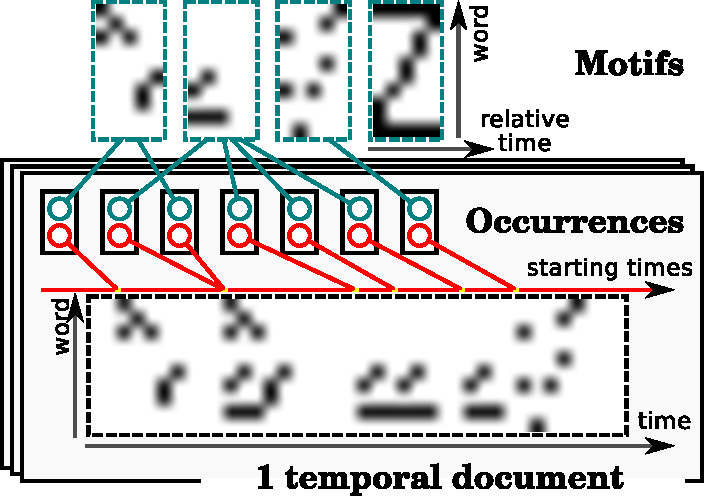
\includegraphics[width=.4\textwidth]{fig/hdlsm}
\caption{In the HDLSM model, a document is seen as a mixture of motif
occurrences. \label{fig:hdlsm}}
\end{figure} \todo{check fig}

The HDLSM model takes as input a set of quantized time series (aka temporal
documents).
More specifically, a time series is represented as a contingency table that
informs, for
each pair $(w, t)$, whether word (or a quantized feature) $w$ was
present in the time series at time index $t$ (in fact, it can also account for
the \emph{amount} of presence of word $w$ at time $t$).

HDLSM is a generative model. Its generative process can be described as
follows:
\begin{enumerate}
\item Generate a list of motifs, each motif $k$ being a 2D probability map
indicating how likely it is that word $w$ occurs at relative time $t_r$ after
the beginning of the motif.
\item For each document $j$, generate a list of occurrences, each occurrence having
a starting time $t_o$ and an associated motif $k$.
\item For each observation $i$ in document $j$:
  \begin{enumerate}
  \item Draw an occurrence from the list,
  \item Draw a pair $(w, t_r)$ from the associated motif,
  \item Generate the observation of word $w$ at time $t = t_o + t_r$.
  \end{enumerate}
\end{enumerate}

As stated above, motifs are represented as probabilistic maps.
Each map is drawn from a Dirichlet distribution.
This model makes intensive use of Dirichlet Processes (DP) to model the
possibly infinite number of motifs and occurrences.

To learn the parameters of the model, Gibbs sampling is used, in which it
is sufficient to re-sample motif assignments for both observations and
occurrences as well as occurrence starting times.
Other variables are either integrated out or deduced, when a deterministic
relation holds.

Our supervised variant relies on the same generative process except that an
extra component is added that maps motifs (denoted $z$)
to classes ($y$) in a supervised learning
context.
Therefore, this mapping needs to be learned and, once the model is trained,
classifying a new instance $\mathbf{x}$ consists in
(i) extracting motif probabilities $P(z | \mathbf{x})$ and
(ii) deriving class probabilities as:

\begin{equation}
    P(y | \mathbf{x}) = \sum_z P(y | z) P(z | \mathbf{x})
\end{equation}

We have used this model in the context of action recognition in
videos~\cite{tavenard:hal-00872048}.
Here, our \emph{words} are quantized spatio-temporal features and each time series
is the encoding of a video in which a single action is performed.
In this context, we show that our
model outperforms standard competitors that operate on the same quantized
features.

\subsection{Two-step Inference for Sequences of Ornstein Uhlenbeck Processes}
\label{sec:oup}

More recently, I have been involved in a project related to the surveillance of
the maritime traffic.
In this context, a major challenge
is the automatic identification of traffic flows from a set of observed
trajectories, in order to derive good management measures or to detect abnormal
or illegal behaviors for example.%
\footnote{This work was part of Pierre Gloaguen's postdoc.
This is joint work with Laetitia Chapel and Chloé Friguet.}

The model we have proposed in this context differs from the one described above
in several aspects:

\begin{itemize}
\item We are not in a supervised setting, we have no labelled data at our disposal
and our goal will rather be to extract meaningful trajectory clusters;
\item We are not looking for motifs to be localized in time series (with
a possible overlap between motifs, as in the method described above) but rather
in the segmentation of trajectories into homogeneous \emph{movement modes};
\item Each movement mode is described using a continuous time model;
\item In order to scale to larger datasets, stochastic variational inference is used
(in place of Gibbs sampling) for inference.
\end{itemize}

\subsubsection{Motivating Use Case}

The monitoring of maritime traffic relies on several sources of data, in a
rising context of maritime big data~\cite{garnier2016exploiting}.
Among these sources lies the Automatic Identification System (AIS), which
automatically collects messages from vessels around the world, at a high
frequency.
AIS data basically consist of GPS-like data, together with the instantaneous
speed and heading, and some vessel specific static information.
These data are characterized by their diversity as they (1) are collected at
different frequencies (2) have different lengths (3) are not necessarily
regularly sampled (4) represent very different behaviors, (5) share common
trends or similar subparts (\emph{movement modes}).

One major challenge in this context is the extraction of movement patterns
emerging from the observed data, considering trajectories that share similar
movement modes.
This issue can be restated from a machine learning point of view as a
large-scale clustering task.
This tasks involves the definition of clustering methods
that can handle such complex data while being efficient on large databases,
and that both cluster trajectories as a whole and detect common
sub-trajectories.

\subsubsection{Model}

We define a parametric framework to model trajectory data,
\emph{i.e.} sequences of geographical positions recorded through time.
The modeling framework aims to account for two levels of heterogeneity possibly
present in trajectory data:

\begin{enumerate}
\item heterogeneity of a vessel's movement within a single trajectory, and
\item heterogeneity between observed trajectories of several vessels.
\end{enumerate}

Following a common paradigm, we assume that a moving vessel's trajectory
is a heterogeneous sequence of patterns that we call \emph{movement modes}.
Different movement modes along a trajectory refer to different ways of moving
in terms of velocity distribution, reflecting different behaviors, activities,
or routes.
It is assumed that a given movement mode can be adopted by several vessels.

As done in~\cite{gurarie2017correlated}, we characterize
movement modes using a specific correlated velocity model, defined in a
continuous-time framework, namely the Ornstein-Uhlenbeck
Process~\cite{uhlenbeck1930theory} (OUP).
One important property of the OUP is that, under mild conditions,
the velocity process is an asymptotically stationary Gaussian Process, which
can be visualized in Figure~\ref{fig:oup}.

\begin{figure}
\centering
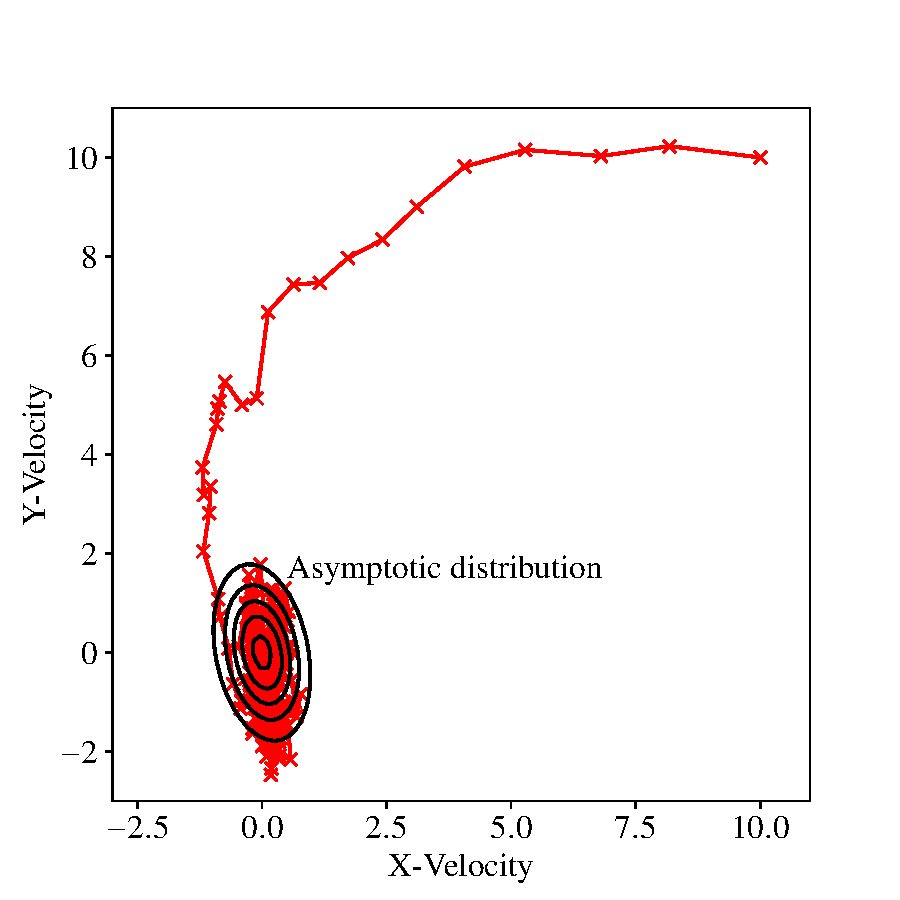
\includegraphics[width=.5\textwidth]{fig/oup}
\caption{Simulation of an OUP process. The starting point is in the
top-right corner and level sets of the asymptotic distribution are shown.
\label{fig:oup}}
\end{figure}

\subsubsection{Parameter estimation}

In order to perform scalable parameter inference and clustering of both
trajectories and GPS observations (into movement modes), we adopt a pragmatic
two step approach that takes advantage of the inherent properties of the OUP:

\begin{enumerate}
\item A first dual clustering is performed based on a simpler independent
Gaussian Mixture Model, in order to estimate potential movement modes and
trajectory clusters: it removes within mode autocorrelation in
the inference, and therefore facilitates the computations, yet it does not rely
on any temporal or sequential information.
Here again, we use a Hierarchical Dirichlet Process as a model for this
two-level clustering, hence allowing for infinite mixtures of both movement
modes and trajectory clusters.
The Gaussian hypothesis in this case is in line with our choice of the OUP as
our velocity process, since the OUP stationary distribution is Gaussian.
\item Among the estimated movement modes, only those meeting a temporal consistency
constraint are kept.
Parameters of these consistent movement modes are then estimated, and used to
reassign observations that were assigned to inconsistent movement modes (\emph{i.e.}
movement modes that do not last long enough to be considered reliable).
It ensures that only trajectory segments for which the stationary distribution
is reached are kept to estimate movement modes.
\end{enumerate}

The resulting consistent movement mode concept allows one to (1) have a good
estimation of OUP parameters within a movement mode (as a consistent sequence
will often be related to a large amount of points) and (2) filter out
"noise" movement modes gathering few observations in a temporally
inconsistent manner.

Parameter estimation for Step 1 described above is performed through stochastic
variational inference (SVI) to allow scalability to large datasets of AIS data,
and movement mode parameter estimation is performed using standard tools from
the OUP literature.

The clustering
step is predominant in the overall computational complexity at inference time,
since the OUP parameter estimation can be performed independently for each
movement mode.
It is quasilinear in the number of
observations and, as stochastic variational inference is used, parts of the
computations involved can easily be distributed.

\subsubsection{Results}

We have provided \href{https://github.com/rtavenar/ushant_ais}{a dataset} of
several
millions of observations in the AIS context.
This dataset is used in~\cite{gloaguen2020} to validate our model qualitatively
(through visual
analysis of extracted movement modes and trajectory clusters) and compare it to
a standard $k$-means clustering.
We intend to make this dataset a reference for future competitive methods to
compare on a
real-world large-scale trajectory dataset.
